\documentclass[10pt]{beamer}

\usetheme{CambridgeUS}
\usepackage[italian]{babel}
\usepackage[latin1]{inputenc}

\usepackage{longtable}
\usepackage{colortbl}
\usepackage{multirow}

\setbeamercovered{transparent}

\title{\textbf{ShirtShop}}
\subtitle{Negozio vendita on-line Magliette Personalizzate}
\author{Sistemi Informativi e Servizi in Rete}

\date{A.A. 2011-2012}

\begin{document}

\begin{frame}
	\maketitle
	Iora Marco 65574\\ Lorenzi Roberta 72361 \\ Piccinelli Andrea 83392\\
\end{frame}

\begin{frame}
	\frametitle{Obiettivi dell'applicazione}
	L'applicazione si propone di:
	\begin{itemize}
		\item <1-> essere una vetrina per la vendita di prodotti (magliette con stampe fronte e/o retro)
		on-line personalizzabili secondo qualunque esigenza
		\item <2-> fornire ai visitatori un'applicazione facile da usare per creare i propri prodotti
		personalizzati anche con stampe inviate dagli stessi clienti 
	\end{itemize}
\end{frame}

\begin{frame}
	\frametitle{Schema gerarchico degli utenti}
	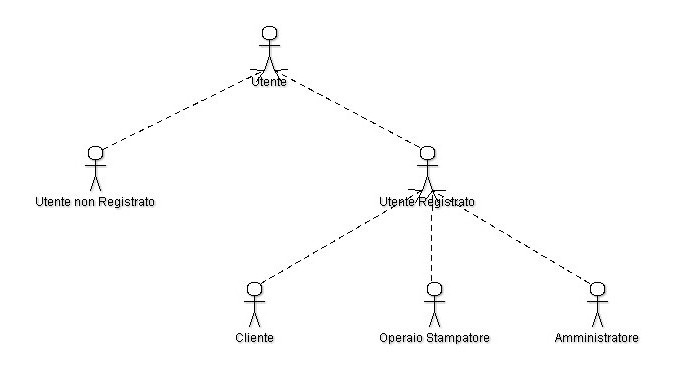
\includegraphics[height= 7cm]{Immagine/GerarchiaUtenti.jpg}
\end{frame}

\begin{frame}
	\frametitle{Diagramma dei casi d'uso: CLIENTE}
	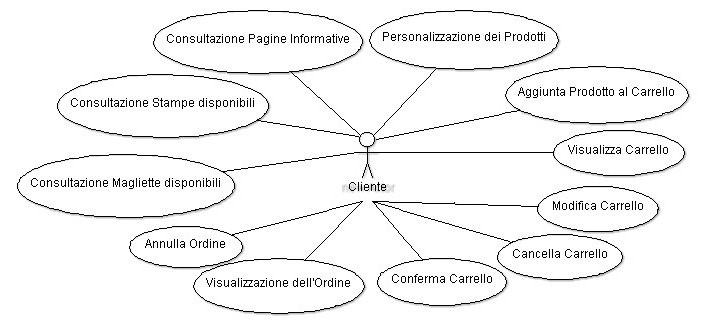
\includegraphics[height=5.5cm]{Immagine/CasoCliente.jpg}
\end{frame}

\begin{frame}
	\frametitle{Diagramma dei casi d'uso: OPERAIO STAMPATORE}
	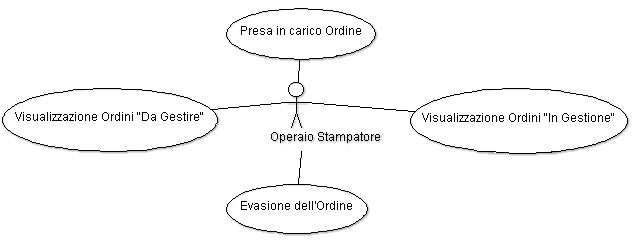
\includegraphics[height=4.5cm]{Immagine/CasoOperaioStampatore.jpg}
\end{frame}

\begin{frame}
	\frametitle{Diagramma dei casi d'uso: AMMINISTRATORE}
	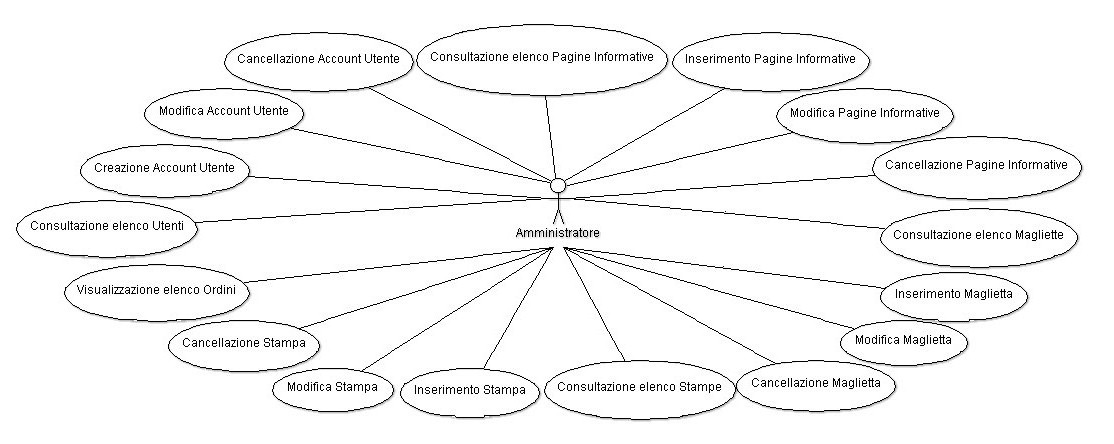
\includegraphics[height=5cm]{Immagine/CasoAmministratore.jpg}
\end{frame}

\begin{frame}
	\frametitle{Dizionario dei Dati}
	I principali oggetti informativi individuati durante l'analisi dei requisiti sono i seguenti:
	\begin{columns}
		\begin{column}{0.4\textwidth}
			\begin{itemize}
				\item Cliente
				\item Operaio Stampatore
				\item Stampa
				\item Tema
				\item Maglietta 
				\item Colore
				\item Sesso
			\end{itemize}
		\end{column}
		\begin{column}{0.4\textwidth}
			\begin{itemize}
				\item Taglia
				\item Foto
				\item Template
				\item Configurazione
				\item Riga di un Ordine
				\item Ordine
				\item Pagina
			\end{itemize}
		\end{column}
	\end{columns}
\end{frame}

\begin{frame}
	\frametitle{Dizionario dei Dati: MAGLIETTA}
			\begin{longtable}{|l|p{0.7\columnwidth}|}
				\hline
				\rowcolor[gray]{.7} \textbf{Nome}& \textbf{Maglietta}\\
				\hline
				Sinonimi & T-shirt \\
				\hline
				Descrizione & Tipo di maglietta disponibile per la personalizzazione in una o pi� delle sue
				caratteristiche e per l'acquisto. Le caratteristiche della maglietta sono la disponibilit�
				in diverse taglie, colori e sesso. Pu� inoltre essere o meno personalizzabile con stampe 
				scelte dal cliente su fronte e/o retro indipendentemente.\\
				\hline
				Istanze Campione & ""StilistaOne PE2011"": Maglietta manica corta 
				di cotone, collezione Primavera-Estate 2011 by StilistaOne, disponibile nelle taglie S e M, 
				nei colori rosso, fucsia e verde a strisce blu orizzontali, taglio femminile.\\
				\hline
			\end{longtable}
\end{frame}
\begin{frame}
	\frametitle{Dizionario dei Dati: MAGLIETTA 2}
			\begin{longtable}{|l|p{0.7\columnwidth}|}
				\hline
				Propriet� & \underline{OID}: chiave univoca dell'entit� considerata\\
				& \underline{Nome(string)}: nome descrittivo della maglietta con il quale questa viene riferita sui
				documenti (ordine, DDT, fattura)\\
				& \underline{Descrizione(text)}: descrizione dettagliata della maglietta con accezioni commerciali e 
				spiegazioni inerenti la maglietta\\
				& \underline{Manica(string)}: tipo di manica della maglietta\\
				& \underline{Collo(string)}: tipo di collo della maglietta \\
				& \underline{StampabileFronte(boolean)}: possibilit� di scelta di una stampa sul fronte della maglietta
				in fase di configurazione\\
				& \underline{StampabileRetro(boolean)}: possibilit� di scelta di una stampa sul retro della maglietta
				in fase di configurazione\\
				& \underline{Materiale(string)}\\
				& \underline{Prezzo(float)}\\
				& \underline{isActive(boolean)}: se true la maglietta � visualizzata dagli utenti finali\\
				\hline
			\end{longtable}
\end{frame}
\begin{frame}
	\frametitle{Dizionario dei Dati: MAGLIETTA 3}
			\begin{longtable}{|l|p{0.7\columnwidth}|}
				\hline
				Relazioni & Maglietta-Colore\\
				& Maglietta-Taglia\\
				& Maglietta-Sesso\\
				& Maglietta-Foto\\
				& Maglietta-Configurazione\\
				\hline
				Componenti & Colore\\
				& Taglia\\
				& Sesso\\
				& Foto\\
				& Stampa\\
				\hline
				Super-concetti & \\
				\hline
				Sotto-concetti & Template\\
				\hline
			\end{longtable}
\end{frame}

\begin{frame}
	\frametitle{Dizionario dei Dati: STAMPA}
	\begin{longtable}{|l|p{0.7\columnwidth}|}
		\hline
		\rowcolor[gray]{.7} \textbf{Nome}& \textbf{Stampa}\\
		\hline
		Sinonimi & Disegno \\
		\hline
		Descrizione & Prototipo di disegno disponibile per essere impresso sulle magliette in vendita
		ai clienti.\\
		\hline
		Istanze Campione &""Gioconda"": Stampa raffigurante la Gioconda di Leonardo da Vinci\\
		& ""Logo Ubuntu"": Stampa raffigurante il logo di Ubuntu\\
		\hline
	\end{longtable}
\end{frame}
\begin{frame}
	\frametitle{Dizionario dei Dati: STAMPA 2}
	\begin{longtable}{|l|p{0.7\columnwidth}|}
		\hline
		Propriet� & \underline{OID}: chiave univoca dell'entit� considerata\\
		& \underline{Nome(string)}: nome identificativo della stampa con il quale questa viene riferita sui 
		documenti (ordine, DDT, fattura)\\
		& \underline{Descrizione(text)}: descrizione dettagliata della stampa con accezioni commerciali e 
		spiegazioni inerenti al disegno, quali ad esempio artista che lo ha realizzato, anno, etc..\\
		& \underline{Anteprima(blob-image)}: anteprima della stampa\\
		& \underline{ImmagineHD(blob-image)}: immagine a grandezza reale della stampa a uso esclusivo degli operai
		stampatori per la realizzazione delle magliette personalizzate\\
		& \underline{PrezzoBase(float)}: prezzo finale della stampa a dimensione massima\\
		& \underline{isActive(boolean)}: se true la stampa � visualizzabile dagli utenti finali\\
		\hline
	\end{longtable}
\end{frame}
\begin{frame}
	\frametitle{Dizionario dei Dati: STAMPA 3}
	\begin{longtable}{|l|p{0.7\columnwidth}|}
		\hline
		Relazioni & Stampa-Template (stampa sul fronte)\\
		& Stampa-Template (stampa sul retro)\\
		& Stampa-Configurazione (stampa sul fronte)\\
		& Stampa-Configurazione (stampa sul retro)\\
		& Stampa-Cliente\\
		& Stampa-Tema\\
		\hline
		Componenti & \\
		\hline
		Super-concetti & \\
		\hline
		Sotto-concetti & \\
		\hline
	\end{longtable}
\end{frame}

\begin{frame}
	\frametitle{Site View}
	Le Site View individuate sono le seguenti:
	\begin{columns}
		\begin{column}{0.4\textwidth}
			\begin{itemize}
				\item \underline{Pubblica} con le seguenti aree:
					\begin{itemize}
						\item Home Page
						\item Prodotti
						\item Informazioni
					\end{itemize}
				\item \underline{Cliente} con le seguenti aree:
					\begin{itemize}
						\item Web Market
						\item Informazioni 
						\item Ordini
						\item Gestione Account
					\end{itemize}
			\end{itemize}
		\end{column}
		\begin{column}{0.4\textwidth}
			\begin{itemize}
				\item \underline{Stampatore} con le seguenti aree:
					\begin{itemize}
						\item Gestione Ordini
						\item Gestione Account
					\end{itemize}
				\item \underline{Amministratore} con le seguenti aree:
					\begin{itemize}
						\item Gestione Accounts
						\item Gestione Informazioni
						\item Gestione Prodotti
						\item Gestione Archivio Ordini
					\end{itemize}
			\end{itemize}
		\end{column}
	\end{columns}
\end{frame}

\begin{frame}
	\frametitle{Site View: CLIENTE}
	\begin{longtable}{|l|p{0.7\columnwidth}|}
		\hline
		\rowcolor[gray]{.9} Site View & \textbf{Cliente}\\
		\hline
		Descrizione & Site view riservata ai clienti del negozio che hanno effettuato login. I clienti
		possono consultare il catalogo dei prodotti (magliette e stampe), personalizzare ed ordinare
		le magliette desiderate. Possono sempre verificare lo stato dei propri ordini sia in gestione
		che gi� evasi. Inoltre possono modificare i propri dati di registrazione ed effettuare il 
		logout dal sito. Infine, cos� come i visitatori, i clienti possono sempre visualizzare le 
		pagine informative dell'azienda.\\
		\hline
		Gruppi d'Utente & Utente Registrato: Cliente\\
		\hline
		Caso d'Uso & ... \\
		\hline
	\end{longtable}
\end{frame}

\begin{frame}
	\frametitle{Site View: CLIENTE Area: WEB MARKET}
	\begin{longtable}{|l|p{0.7\columnwidth}|}
		\hline
		\rowcolor[gray]{.9} & \textbf{Site View Area: Web Market}\\
		\hline
		Nome Area & Web Market\\
		\hline
		Descrizione Area & Permette la consultazione del catalogo, la selezione di una maglietta e 
		la sua ""configurazione"", con in particolare la possibilit� di scegliere le eventuali stampe
		tra le disponibili o inviare al sistema le proprie mediante upload. E' possibile in questo 
		modo comporre il proprio carrello della spesa e, una volta definitivo, darne conferma 
		trasformandolo in un ordine.\\
		\hline
		Oggetti & Maglietta, Template, Stampa, Configurazione, Ordine\\
		\hline
		Priorit� & Alta\\
		\hline
	\end{longtable}
\end{frame}

\begin{frame}
	\frametitle{Site View: CLIENTE Area: INFORMAZIONI e ORDINI}
	\begin{longtable}{|l|p{0.7\columnwidth}|}
		\hline
		\rowcolor[gray]{.9} & \textbf{Site View Area: Informazioni}\\
		\hline
		Nome Area & Informazioni\\
		\hline
		Descrizione Area & Permette di visualizzare le pagine informative predisposte dall'amministratore.\\
		\hline
		Oggetti & Pagina\\
		\hline
		Priorit� & Bassa\\

		\hline
		\rowcolor[gray]{.9} & \textbf{Site View Area: Ordini}\\
		\hline
		Nome Area & Ordini\\
		\hline
		Descrizione Area & Il cliente, mediante questa area, pu� verificare lo stato e, pi� in generale, 
		l'archivio storico dei suoi ordini. Per ordini gi� confermati dal clienti, ma non ancora 
		presi in carico, esiste qui la possibilit� di annullarli.\\
		\hline
		Oggetti & Ordine, Maglietta, Configurazione, Stampa\\
		\hline
		Priorit� & Media\\
		\hline
	\end{longtable}
\end{frame}

\begin{frame}
	\frametitle{Site View: CLIENTE Area: GESTIONE ACCOUNT}
	\begin{longtable}{|l|p{0.7\columnwidth}|}
		\hline
		\rowcolor[gray]{.9} & \textbf{Site View Area: Gestione Account}\\
		\hline
		Nome Area & Gestione Account\\
		\hline
		Descrizione Area & All'interno di quest'area l'utente pu� controllare ed eventualmente modificare
		i propri dati identificativi ed anagrafici.\\
		\hline
		Oggetti & Utente, Cliente\\
		\hline
		Priorit� & Bassa\\
		\hline
	\end{longtable}
\end{frame}

\begin{frame}
	\frametitle{Site View: STAMPATORE}
	\begin{longtable}{|l|p{0.7\columnwidth}|}
		\hline
		\rowcolor[gray]{.7} \multicolumn{2}{|c|}{\textbf{Presentazione della Site View}}\\
		\hline
		\rowcolor[gray]{.9} Site View & \textbf{Stampatore}\\
		\hline
		Descrizione & Site view dedicata all'operaio stampatore che pu�, in queste pagine, gestire 
		direttamente gli ordini dei clienti.\\
		\hline
		Gruppi d'Utente & Utente Registrato: Operaio Stampatore\\
		\hline
		Caso d'Uso & ...\\
		\hline
	\end{longtable}
\end{frame}

\begin{frame}
	\frametitle{Site View: STAMPATORE Area: GESTIONE ORDINI e GESTIONE ACCOUNT}
	\begin{longtable}{|l|p{0.7\columnwidth}|}
		\hline
		\rowcolor[gray]{.9} & \textbf{Site View Area: Gestione Ordini}\\
		\hline
		Nome Area & Gestione Ordini\\
		\hline
		Descrizione Area & Tramite le pagine di quest'area, � possibile visualizzare l'elenco degli 
		ordini in attesa di essere gestiti e quelli gi� presi in carico dall'operaio stampatore
		che ha effettuato login. L'utente pu� visualizzare il dettaglio dei singoli ordini e gestirne
		lo stato, dalla presa in carico alla spedizione.\\
		\hline
		Oggetti & Ordine, RigaOrdine, Configurazione, Maglietta, Stampa, Cliente\\
		\hline
		Priorit� & Alta\\
		\hline
		\rowcolor[gray]{.9} & \textbf{Site View Area: Gestione Account}\\
		\hline
		Nome Area & Gestione Account\\
		\hline
		Descrizione Area & All'interno di quest'area l'utente pu� controllare ed eventualmente modificare
		i propri dati identificativi\\
		\hline
		Oggetti & Utente, Operaio Stampatore\\
		\hline
		Priorit� & Bassa\\
		\hline
	\end{longtable}
\end{frame}

\begin{frame}
	\frametitle{Oggetti core e sotto-schemi core}
	\begin{center}
		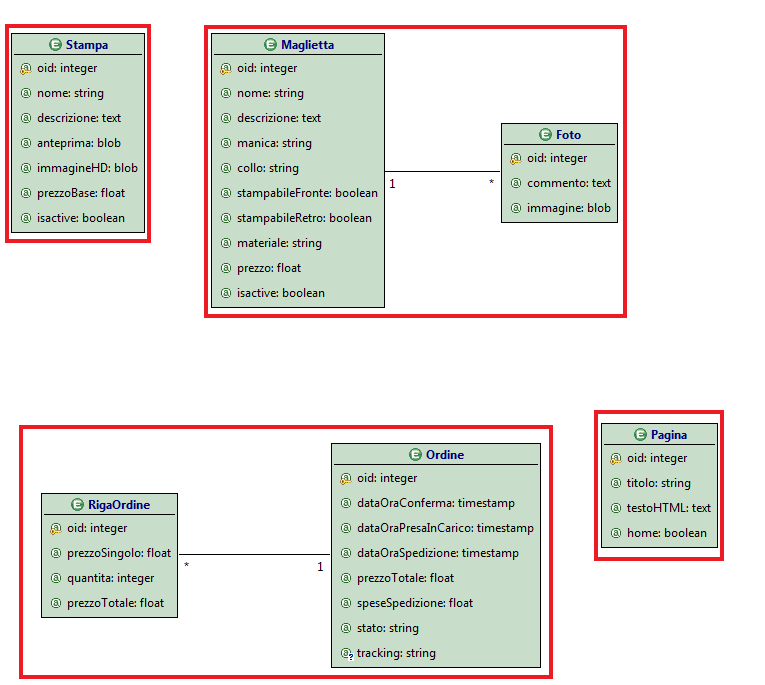
\includegraphics[height=7.5cm]{Immagine/Core.png}
	\end{center}
\end{frame}

\begin{frame}
	\frametitle{Sotto-schema di interconnesione}
	\begin{center}
		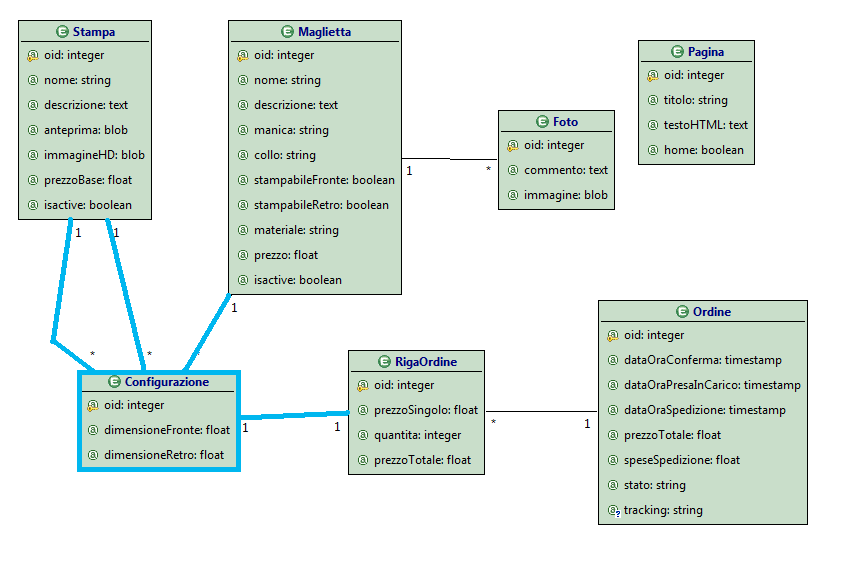
\includegraphics[height=7.5cm]{Immagine/Interconnessione.png}
	\end{center}
\end{frame}

\begin{frame}
	\frametitle{Sotto-schemi di accesso}
	\begin{center}
		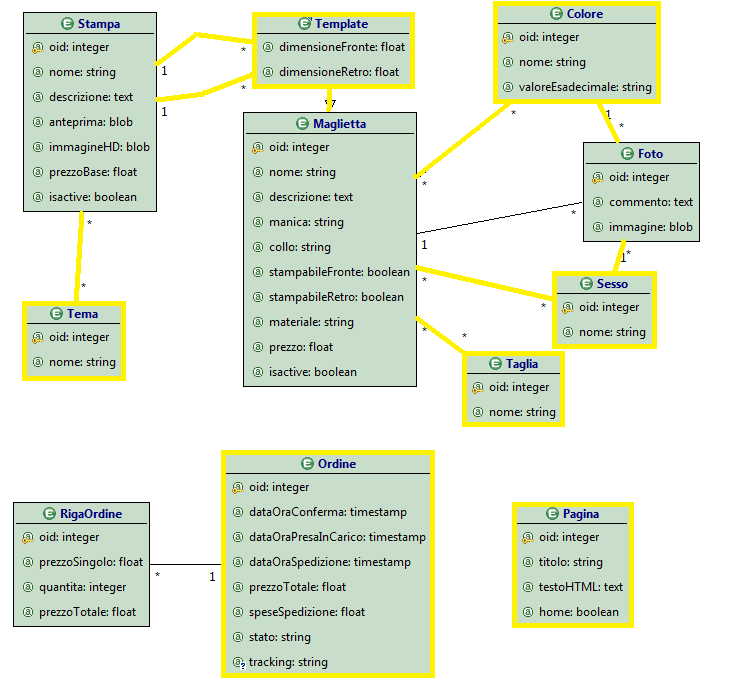
\includegraphics[height=7.5cm]{Immagine/Accesso.png}
	\end{center}
\end{frame}

\begin{frame}
	\frametitle{Sotto-schema di personalizzazione}
	\begin{center}
		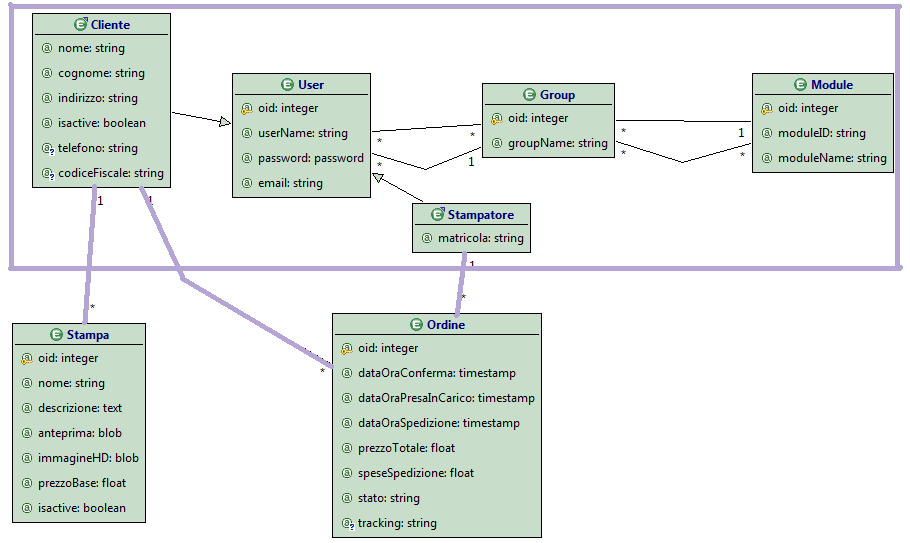
\includegraphics[height=6.5cm]{Immagine/Personalizzazione.png}
	\end{center}
\end{frame}

\begin{frame}
	\frametitle{Schema completo dei dati}
	\begin{center}
		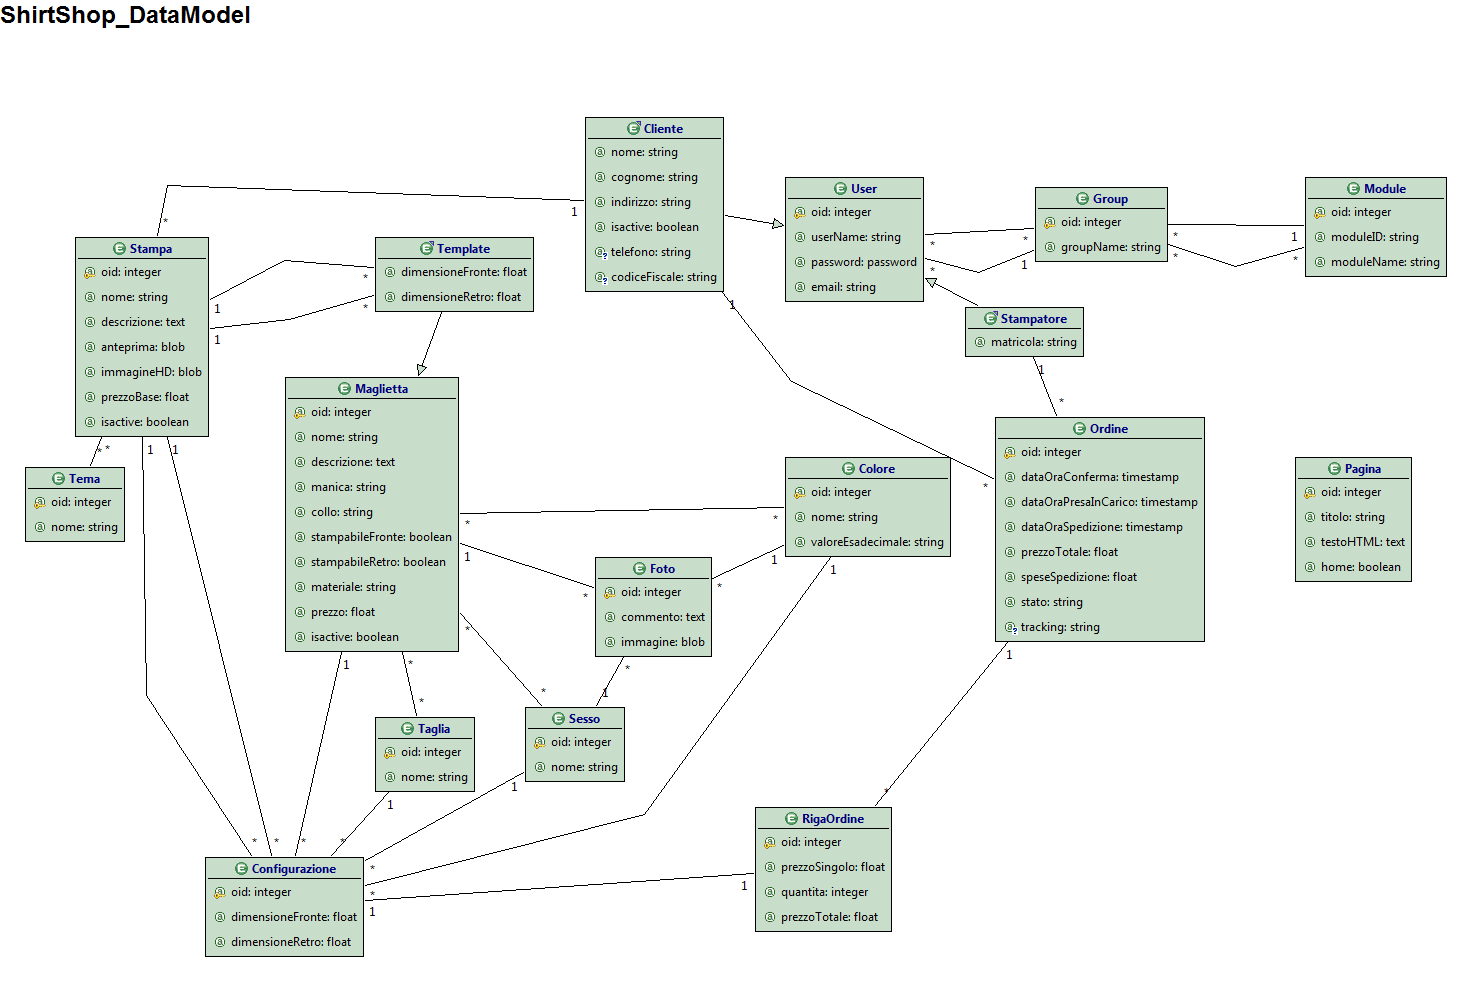
\includegraphics[height=7.5cm]{Immagine/SchemaCompletoDati.png}
	\end{center}
\end{frame}

\end{document}